% \documentclass[aps,pra,floatfix,amsmath,amssymb,preprint,eqsecnum,nofootinbib,superscriptaddress]{revtex4-1}
\documentclass{article}
% \usepackage{graphicx}% Include figure files
% \usepackage{dcolumn}% Align table columns on decimal point
% \usepackage{bm}% bold math
% \usepackage{epstopdf}
% \usepackage{framed}
% %\usepackage{showkeys}
% \usepackage{setspace}   % controllabel line spacing
% %% If an increased spacing different from one-and-a-half or double spacing is
% %% required then the spacing environment can be used.  The spacing environment
% %% takes one argument which is the baselinestretch to use,
% %%         e.g., \begin{spacing}{2.5}  ...  \end{spacing}
% \renewcommand{\labelitemii}{$\star$} %change bulletpoint symbol to star
% \usepackage[toc,page]{appendix}

\usepackage[utf8]{inputenc}
% \usepackage{natbib}
% \usepackage[
% backend=biber,
% style=alphabetic,
% sorting=ynt
% ]{biblatex}

% \addbibresource{refs.bib}

% \linespread{1.15} %line spacing
% \pagestyle{plain} % page numbers on bottom
\newcommand{\cH}{\mathcal{H}}
% \newcommand{\beq}{\begin{equation}} broken?
\newcommand{\eeq}{\end{equation}}
% \newcommand{\ba}{\begin{array}{ccc}} broken?
\newcommand{\ea}{\end{array}}
\newcommand{\half}{\frac{1}{2}}
\newcommand{\nn}{\nonumber}
 \renewcommand{\d}{\partial}
% \def\bea{\begin{eqnarray}} broken?
\def\eea{\end{eqnarray}}
\def\rar{\rightarrow}
\def\la{\lambda}
\def\al{\alpha}
\def\prl{\parallel}
\def\ga{\gamma}
\def\om{\omega}
\def\psit{\tilde{\psi}}
\def\Tr{ {\rm Tr} }
\def\<{\langle}
\def\>{\rangle}
\def\mx{\mathrm{x}}
\def\mm{\mathrm{m}}
\def\bZ{\mathbb{Z}}
\def\bR{\mathbb{R}}
\def\bC{\mathbb{C}}
\def\cL{\mathcal{L}}
\def\cA{\mathcal{A}}
\def\cO{\mathcal{O}}
\usepackage{amsmath}
\usepackage{comment}
\usepackage{amssymb}
\usepackage{amsthm}
\newtheorem{thm}{Theorem}
\newtheorem{lemma}{Lemma}
\newtheorem{prop}{Proposition}
\newtheorem{conj}{Conjecture}
\theoremstyle{definition}
\newtheorem{defn}{Definition}
\newtheorem{q}{Question}
%\usepackage{feynmp}
\usepackage{color}
\usepackage{tikz-cd}
\usepackage{comment}
\newcommand{\de}[1]{\textcolor{red}{DE: #1}}

\newcommand{\ket}[1]{|#1\rangle}
\newcommand{\eqnref}[1]{Eq.~(\ref{#1})}
\newcommand{\U}{\mathrm{U}}

\usepackage{tikz}

% \title{Anomalies and Bosonization}

% \author{Ryan Thorngren}


% \date{\today}



\begin{document}

% \maketitle

\begin{abstract}
Discrete spin structures.

\noindent



\end{abstract}


\section{Stiefel-Whitney Classes}

\subsection{Some Discrete Topology}

\subsection{Discrete Morse Flows}

In this section we describe some aspects of Robin Forman's discrete Morse theory \cite{FORMAN199890}. Our main application is the construction of a discrete Morse flow on the barycentric subdivision $X^b$ whose unstable cells are exactly the original cells of $X$. This Morse flow depends on a branching structure of $X$.

We define a discrete flow $V$ to be a collection of pairs $\sigma_k \to \tau_{k+1}$ where $\sigma_k$ is a $k$-cell on the boundary of the $k+1$-cell $\tau_{k+1}$ such that each cell appears in \textit{at most} one pair. A $V$-path is a sequence of pairs
\[\sigma_k^0 \to \tau_{k+1}^0 > \sigma_k^1 \to \tau_k^1 > \cdots > \tau_k^m \to \sigma_k^m,\]
such that $\sigma_k^j \neq \sigma_k^{j+1}$ (no backtracking). $V$ is called a discrete Morse flow if it has no cyclic $V$-paths, ie. $\sigma^0_k \neq \sigma^m_k$ for all $V$-paths. In this case, one can actually define $V$ as a discrete gradient of a function. We will not pursue this here, however.

Given a discrete Morse flow $V$, we define a critical cell to be any cell which does not occur in one of the pairs of $V$. For each critical cell $\sigma^*_k$ of the original CW complex, we call the union of $V$-paths beginning on the boundary of $\sigma^*_k$ the unstable manifold of $\sigma^*_k$, while the union of all $V$-paths ending on the boundary of $\sigma^*_k$ we call the stable manifold of $\sigma^*_k$. $X$ is both a union of all unstable manifolds of critical cells and a union of all stable manifolds of critical cells. That $V$ has no cyclic paths implies that these cells are all polyhedra. Thus, either of these unions define a CW coarsening of $X$.

% \thm{\emph{Branching Morse Flow}\label{thm:branchingmorse} A branching structure on a combinatorial CW complex defines a Morse flow on its barycentric subdivision whose unstable cells are the cells of the original triangulation.
% }

% \thm{A branching structure on a combinatorial CW complex defines a Morse flow on its barycentric subdivision whose unstable cells are the cells of the original triangulation.}

\begin{thm} \textbf{Branching Morse Flow}
A branching structure on a combinatorial CW complex defines a Morse flow on its barycentric subdivision whose unstable cells are the cells of the original triangulation.
\end{thm}

\begin{proof}


For convenience we first describe the critical simplices, for simplicity focusing on a triangulated space $X$. They correspond to the $k$-simplices of $X$ $\sigma_k = (i_0 \cdots i_k)$ of $X$ by
\begin{equation}\label{e:critsimplices}
    (i_0 \cdots i_k) \mapsto ((i_0) < (i_0 i_1) < \cdots < (i_0 \cdots i_k))
\end{equation}
where we use the branching structure to order $i_0 < \cdots < i_k$. We denote a subsequence of this kind, namely of the form
\[(i_0 \cdots i_m) < (i_0 \cdots i_{m+1}) < \cdots < (i_0 \cdots i_{m+l})\]
such that $i_0 < \cdots < i_{m+l}$ a \emph{frozen} sequence.



We extend a total ordering of vertices of $X$ to a total ordering on all the simplices of $X^b$ by extending each $k$-simplex $(i_0 \cdots i_k)$ to a list of length $n+1$:
$(i_0 \cdots i_k) \mapsto (i_k, \ldots, i_0, \infty, \ldots, \infty)$
and then using lexicographical ordering. We denote this ordering $\lhd$ and call it the simplex ordering. In this ordering, the largest simplex is the vertex of highest degree, followed by other simplices containing this vertex. Then it goes on to the vertex of next highest degree, followed by all the simplices containing this one but not the highest one, and so on.

Given a $k$-simplex
\[(\sigma_{i_0} < \sigma_{i_1} < \cdots < \sigma_{i_k}),\]
we let $j$ be the least $j$ such that
\[\sigma_{i_{j+1}} < \cdots < \sigma_{i_k}\]
is frozen. We then look for simplices $\rho$ which may be inserted in the initial ``unfrozen" subsequence
\[\sigma_{i_0} < \cdots < \sigma_{i_j}\]
such that
\[\sigma_{i_m} \lhd \rho\]
for all $m\le j$. We call these \emph{admissible insertions}. We look for the largest possible $\rho$ with an admissible insertion and insert it to form a $k+1$-simplex
\[(\sigma_{i_0} < \cdots \sigma_{i_l} < \rho < \sigma_{i_{l+1}} \cdots < \sigma_{i_k}).\]
Note that the final frozen subsequence of this $k+1$-simplex is the same as our original $k$-simplex. Indeed, this is clear if $l \neq j$. However, if $l = j$, then we have a situation like
\[\rho < (i_0 \cdots i_m) < \cdots,\]
where $i_0 < \cdots < i_m$ and if $\rho$ were to be added to the frozen subsequence then we would necessarily have
\[\rho = (i_0 \cdots i_{m-1}),\]
but there are larger insertions. Thus, the final frozen subsequence stays the same, and since there is no bigger admissible insertion than $\rho$ in the intial unfrozen subsequence, our $k+1$-simplex so constructed admits no admissible insertions of its own. Therefore, the set of pairs
\[(\sigma_{i_0} < \sigma_{i_1} < \cdots < \sigma_{i_k}) \to (\sigma_{i_0} < \cdots \sigma_{i_l} < \rho < \sigma_{i_{l+1}} \cdots < \sigma_{i_k})\]
defines a discrete Morse flow on $X^b$.

Note that the last element of any $k$-simplex forms a frozen subsequence of length 1, so $\rho$ is always inserted to the left of $\sigma_k$. It follows that this Morse flow pairs simplices of $(X_m)^b$ with other simplices of $(X_m)^b$ for all $m$. That is, it preserves the skeleton of $X$, and can be considered as glued together from this same Morse flow constructed $n$-simplex by $n$-simplex.

It remains to show that the $k$-simplices of \eqref{e:critsimplices} are precisely the critical simplices of this Morse flow. These sequences are frozen and have no admissible insertions so they are critical. We need only show that they are the only critical simplices. Suppose a sequence
\[\sigma_{i_0} < \cdots < \sigma_{i_k}\]
admits no admissible insertions. If this sequence is completely frozen, it must be one of the $k$-simplices of $\eqref{e:critsimplices}$, otherwise, $\sigma_{i_0}$ is not a vertex and it admits an insertion at the left. 

Otherwise, we let
\[\sigma_{i_0} < \cdots < \sigma_{i_m}\]
be the initial unfrozen subsequence. Let $\sigma_{i_l}$ be the largest in the simplex ordering among these. Suppose if we drop $\sigma_{i_l}$ from the sequence, that it admits an admissible insertion of a $\rho$ which is bigger than $\sigma_{i_l}$. The only way this can be is if $\rho < \sigma_{i_l}$, in which case $\rho$ is an admissible insertion in the original sequence. Otherwise, $\sigma_{i_l}$ is the largest admissible insertion of the sequence obtained by dropping $\sigma_{i_l}$, so again the sequence is not critical.

For more general combinatorial CW complexes, a construction like the above is also possible, except now the dimensions of the cells of $X$ are not fixed to their number of vertices (although they can still be described by their set of vertices) and this makes the notation especially cumbersome. In this more general case, the construction of the flow is identical except for the definition of a frozen sequence. A frozen sequence is a sequence of cells
\[V_1 < \cdots < V_k\]
such that $\dim V_{j+1} = \dim V_j + 1$ and $V_j$ is the least cell of its dimension in the cell ordering of $V_{j+1}$.
\end{proof}



% It's also possible to derive our Morse flow from a Morse function on the standard $n$-simplex $\Delta^n$, formed as the convex hull of orthonormal basis vectors. Using that coordinate system we consider the linear function
% \[f(x_0,\ldots, x_n) = x_0 + a x_1 + a^2 x_2 + \cdots + a^n x_n\]
% for $a$ a positive real number. We assign values to simplices of $\Delta^n$ by the value of $f$ at their centroids. It is easy to check that for $a \gg 1$ the Morse flow of this function as defined by Forman agrees with our combinatorial description above.

\begin{figure}
    \centering
    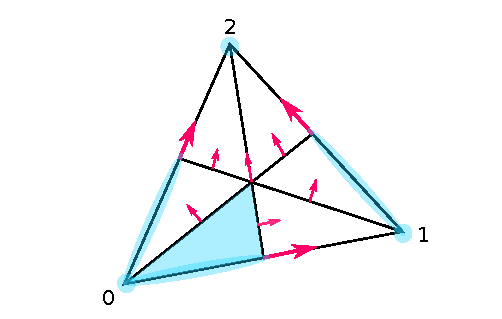
\includegraphics{barycentric-morse-flow.pdf}
    \caption{A picture of the branching Morse flow on a triangle $(012)$, with critical simplices highlighted in blue.}
    \label{fig:morse-flow}
\end{figure}

% Note that the barycentric subdivision $X^b$ has a natural branching structure which defines a Morse flow on the second barycentric subdivision $X^{bb}$. So $X^{bb}$ has a natural Morse flow. This explains why some combinatorial topology constructions use $X^{bb}$. Throughout however we will use the above Morse flow to pass from $X^b$, which has many nice properties, back to $X$.


% First of all, we pair the vertex corresponding to the top simplex of $\Delta^m$
% \[((0 \cdots m)) \to ((m) < (0 \cdots m)).\]

% Consider a $k$-simplex of the interior of $\Delta^{mb}$:
% \[(\sigma^0 < \cdots < \sigma^k = \Delta^m).\]

% We define an ordering on $k$-simplices of $\Delta^m$ by extending each $k$-simplex $(i_0 \cdots i_k)$ to a list of length $m+1$:
% $(i_0 \cdots i_k) \mapsto (i_k, \ldots, i_0, \infty, \ldots, \infty)$
% and then using lexicographical ordering. We denote this ordering $\lhd$. Our Morse flow consists of pairs
% \[(\sigma^0 < \cdots < \sigma^{l-1} < \sigma^{l+1} < \cdots \sigma^k) \to (\sigma^0 < \cdots < \sigma^k),\]
% where $\sigma^{>l} \lhd \sigma^l \lhd \sigma^{<l}$.


% We begin with the 0-simplices $(\sigma_k)$ of $\Delta^{n b}$, which correspond to $k$-simplices $\sigma_k$ of $\Delta^n$. All of those corresponding to $k = 0$ will be critical while the rest will be paired with an edge of $\Delta^{n b}$. Edges meeting $(\sigma_k)$ correspond to 2-chains either $(\sigma_k < \tau)$ or $(\tau < \sigma_k)$. Of the latter (which requires $k>0$) we have those for which $\tau$ is a vertex of $\Delta^n$. We choose our Morse flow to contain the pair
% \[(\sigma_k) \to (v < \sigma_k)\]
% where $v$ is the vertex of highest degree on the boundary of $\sigma_k$. Equivalently we can say that we choose the pair
% \[(\sigma_k) \to (\tau < \sigma_k)\]
% where $\tau$ is the highest possible simplex in the simplex ordering.

% Now we proceed to the 1-simplices $(\tau_j < \sigma_k)$. If $j > 0$ we again choose the highest vertex of


% Those with $j = 0, k = 1$ at this point will either be paired in the Morse flow or critical. We consider then 1-simplices with $j > 0$. Of the 2-simplices meeting these there are those of the form $(v < \tau_j < \sigma_k)$ where $v$ is a vertex of $\Delta^n$. We choose our Morse flow to contain the pair
% \[(\tau_j < \sigma_k) \to (v < \tau_j < \sigma_k)\]
% where $v$ is the vertex of highest degree on the boundary of $\tau_j$.

% By now the pattern should be clear. Our Morse flow is the set of pairs
% \[(\sigma^1 < \cdots < \sigma^m) \to (v < \sigma^1 < \cdots < \sigma^m)\]
% where $v$ is the vertex of highest degree on the boundary of $\sigma^0$. One sees that so long as $\sigma^0$ is not a vertex, the $m+1$-simplex on the right is uniquely defined.

\subsection{Branching Morse Flow and Duality}

\subsection{Halperin-Toledo Framing}

In this section, we describe a framing with singularities that was constructed on a barycentric subdivision of a PL $n$-manifold by Whitney \cite{whitneysphere} and Halperin and Toledo \cite{HalperinToledo}, and explain how to extend it to an arbitrary PL $n$-manifold with branching structure. This makes precise our intuition that a branching structure plays the role of a local coordinate system in the world of combinatorial manifolds.

Let $X$ be a PL $n$-manifold with branching structure. We choose a PL embedding of $X$ into some $\mathbb{R}^N$, meaning that all $k$-simplices of $X$ are embedded as simplices inside an affine $k$-subspace of $\mathbb{R}^N$. If $x \in \sigma = (v_0 \ldots v_k) \in X_k$, ordered using the branching structure, we can write
\[\vec x = \sum_{0 \le j \le k} \lambda_{v_j}(x)\ \vec v_j,\]
where we use vector notation to emphasize that we are using the PL embedding. For each vertex $v \in X_0$ function $\lambda_v$ can be extended to a continuous function on $X$ by $\lambda_v(x) = 0$ whenever $x$ is not in the star of $v$.

Further, for every vertex $v$ we can define a vector field on the star of $v$ called the radial vector field which points radially into $v$, vanishing only at $v$. We denote this vector field $R_v$.

We define the \emph{Halperin-Toledo vector fields} by
\[F_k(x) = \sum_{(v_0\ldots v_k) \in X_k} \lambda_{v_0}(x) \cdots \lambda_{v_k}(x)\ R_{v_k}(x).\]
When $X$ is a barycentric subdivision with the ascending branching structure, this reduces to the definition of the ``fundamental vector fields" of Halperin-Toledo, but they are more general.

These have some important properties (see \cite{HalperinToledo}):
\begin{lemma} The Halperin-Toledo vector fields $F_k$ have the following properties:
\begin{itemize}
    \item $F_k$ are continuous vector fields on $X$, and smooth on each simplex.
    \item $F_k(x) = 0$ for all $x$ in the $k-1$-skeleton.
    \item For $x$ in the interior of a $k$-simplex, $F_1(x),\ldots,F_k(x)$ is a basis for $T_x X$.
\end{itemize}
\end{lemma}

Observe that $F_1$ is our branching Morse flow. For instance, consider the 1-simplex in $\mathbb{R}^N$ with vertices $\vec v_0$ and $\vec v_1$. We can coordinatize this 1-simplex along the branching structure using $\vec x(t) = (1-t) \vec v_0 + t \vec v_1$. In these coordinates, $\lambda_{v_0}(t) = 1-t$ and $\lambda_{v_1}(t) = t$. Further, we see that the radial vector fields are
\[R_{v_0}(t) = t (\vec v_0 - \vec v_1)\]
\[R_{v_1}(t) = (1-t) \vec v_1 - \vec v_0.\]
We check indeed,
\[(1-t) R_{v_0}(t) + t R_{v_1}(t) = 0 \qquad \forall t.\]
Now we see
\[F_1(t) = t(1-t) (\vec v_1 - \vec v_0)\]
describes a monotonic flow from $v_0$ to $v_1$ which fixes these points.

For a 2-simplex spanned by $\vec v_0, \vec v_1, \vec v_2$, we choose right triangle coordinates
\[\vec x(s,t) = (1- s - t)\vec v_0 + s \vec v_1 + t \vec v_2,\]
so that
\[\lambda_{v_0}(s,t) = 1-s-t\]
\[\lambda_{v_1}(s,t) = s\]
\[\lambda_{v_2}(s,t) = t.\]
For any coordinates, the radial vector fields are
\[R_{v_0}(s,t) = \lambda_{v_1}(s,t) (\vec v_0 - \vec v_1) + \lambda_{v_2}(s,t) (\vec v_0 - \vec v_2)\]
\[R_{v_1}(s,t) = \lambda_{v_0}(s,t) (\vec v_1 - \vec v_0)+ \lambda_{v_2}(s,t) (\vec v_1 - \vec v_2)\]
\[R_{v_2}(s,t) = \lambda_{v_0}(s,t)(\vec v_2 - \vec v_0) + \lambda_{v_1}(s,t)(\vec v_2 - \vec v_1),\]
and therefore
\[F_1 = \lambda_{v_0} \lambda_{v_1} R_{v_1} + \lambda_{v_1} \lambda_{v_2} R_{v_2} + \lambda_{v_0} \lambda_{v_1} R_{v_2}.\]
For $N = 2$, $v_0 = (0,0)$, $v_1 = (1,0)$, $v_2 = (0,1)$, we have
\[R_{v_0} = (-x,-y)\]
\[R_{v_1} = (1-x,-y)\]
\[R_{v_2} = (-x,1-y)\]
and
\[F_1 = ((x + y - 1)(x - 1)x + x(y - 1)y, (x + y - 1)xy + y(y - 1)^2),\]
\[F_2 = xy(x+y-1) \cdot (x, y - 1).\]
Observe how $F_2$ vanishes on the lines $x+y = 1$, $x = 0$, and $y = 0$ which bound the 2-simplex. This vector field has appeared in the physics literature, eg. \cite{gaiottokapustin} in the study of discrete spin structures.

It is a corollary of the lemma that the Halperin-Toledo vector fields define a trivialization of the tangent bundle away from the $n-1$-skeleton. Along the $n-1$-skeleton, $F_n$ vanishes and the rest are linearly indepedent away from the $n-2$-skeleton, and so on. In this way, a branching structure nicely defines a ``framing with singularities" of $X$, which justifies its ubiquity in the theory.

Now we define what we call the \emph{discrete Halperin-Toledo Morse flows}, $f^k$. Let $X$ be a PL $n$-manifold with branching structure. $f^1$ is defined to be the branching Morse flow. To define $f^2$, we will take the subflow $f' \subset f^1$ which is trivial on the 1-skeleton $X_1 \subset X^b$. Then, in the interior of every $j$-simplex, we will apply the permutation to $f'$ which exchanges the 1st and 2nd vertex. This defines a discrete Morse flow on $X^b$. To construct $f^k$, we take the subflow of $f^{k-1}$ which is trivial on the $k-1$-skeleton $X_{k-1} \subset X^b$, and in the interior of all higher simplices we apply the permutation exchanging the $k-1$st and $k$th vertices. We will phrase a precise conjecture that we expect these vector fields to satisfy in Chapter \ref{c:obs}.

\subsection{Stiefel-Whitney Cocycles}

\section{Orientations}

\section{Spin Structures on Vector Bundles}

In this section we give six different equivalent definitions of spin structure.

Let $X$ be a topological space with an oriented rank $n$ real vector bundle $V$, $P(V)$ the associated principle $SO(n)$ bundle of oriented orthogonal frames. That is, the fiber of $P(V)$ over $x \in X$ consists of all oriented orthonormal bases of the fiber of $V$ over $x$, which is isomorphic to $\bR^n$. $SO(n)$ acts naturally on these bases by its action on $\bR^n$, transitively and without fixed points. Therefore the fibers of $P(V)$ may be non-canonically identified with $SO(n)$ after choosing a fixed basis of each fiber.

The group $SO(n)$ admits a double cover by the ``spin group" $Spin(n)$, which is also connected. Some special cases include $Spin(1) = \bZ_2$, $Spin(2) = U(1)$, $Spin(3) = SU(2)$. 
\begin{defn}
A \emph{spin structure} on $V$ is a double cover of the frame bundle $S(V) \to P(V)$ which over a fiber, non-canonically identified with $SO(n)$, is equivalent to the double cover $Spin(n) \to SO(n)$.
\end{defn}
Using basic covering space theory \cite{Hatcher}, which identifies $H^1(Y,\bZ_2)$ as the group of double covers of $Y$, we can begin to derive several equivalent definitions:
\begin{defn}
A spin structure is an element $\hat \eta \in H^1(P(V),\bZ_2)$ which restricts to the generator of $H^1(F,\bZ_2)$ where $F \sim SO(n)$ is a fiber.
\end{defn}
Now let us define an $V$-framed curve $\hat\gamma$ as a simple closed curve $\gamma \subset X$ together with a framing of $V|_\gamma$, ie. a lift to $\hat \gamma \subset P(V)$. Using the universal coefficient theorem $H^1(P(V),\bZ_2) = \hom(H_1(P(V),\bZ),\bZ_2),$ we also obtain
\begin{defn}
A spin structure is an assignment $\hat \eta(\hat\gamma) \in \bZ_2$ to $V$-framed curves such that:
\begin{itemize}
    \item If $\hat\gamma$ and $\hat\gamma'$ are isotopic then $\hat \eta(\hat \gamma) = \hat \eta(\hat \gamma')$.
    \item If $\hat\gamma$ bounds a disc in $X$ but its $V$-framing does not extend to the disc then $\hat \eta(\gamma) = 1$ mod 2.
\end{itemize}
\end{defn}
This definition was used in \cite{wilsonlines} to describe Wilson lines of spinning particles.

We can also describe $V$ by its classifying map $f_V:X \to BSO(n)$, by which $V$ is isomorphic to the pullback along $f_V$ of the universal bundle over $BSO(n)$. $BSO(n)$ is the space of $n$-dimensional linear subspaces of $\bR^\infty$, and the universal bundle is the sub-bundle of the constant $\bR^\infty$ whose fiber over a point representing an $n$-dimensional linear subspace of $\bR^\infty$ is that very subspace (this is sometimes called the tautological bundle). Likewise there is a fibration $BSpin(n) \to BSO(n)$, where $BSpin(n)$ is constructed in \cite{}. We can phrase our definition in terms of $f_V:$
\begin{defn}
A spin structure is a homotopy class of lifting of $f_V$ to $BSpin(n)$.
\end{defn}
This follows from the fact that under the fibration $BSpin(n) \to BSO(n)$, the pullback of the universal bundle over $BSO(n)$ to $BSpin(n)$ admits a canonical spin structure. Conversely, the double cover of the frame bundle $S(V)$ is a principal $Spin(n)$ bundle, and therefore classified by such a map to $BSpin(n)$ which lifts $f_V$.

The fibration $BSpin(n) \to BSO(n)$ is in fact a principal $B\bZ_2$ bundle, and therefore has a classifying map of its own:
\[w_2:BSO(n) \to B^2 \bZ_2.\]
We call this map $w_2$ because it defines the 2nd Stiefel-Whitney class of the universal bundle over $BSO(n)$. Indeed, recall that cohomology classes in 
\[H^2(BSO(n),\bZ_2)\]
are equivalent to homotopy classes of such maps. Likewise, $f_V \circ w_2$ defines the 2nd Stiefel-Whitney class of $V$. Moreover, $f_V \circ w_2$ classifies a principal $B\bZ_2$ bundle over $X$, which leads us to another equivalent definition:
\begin{defn}
A spin structure is a homotopy class of sections of the principal $B\bZ_2$ bundle classified by $f_V \circ w_2$.
\end{defn}

This last definition implies that there is an \emph{obstruction class} which characterizes the existence of a spin structure. Indeed, a principal bundle admits a section iff it is trivial. Therefore, we have:
\begin{thm}
The oriented vector bundle $V$ admits a spin structure iff the 2nd Stiefel-Whitney class
\[[w_2(V)] := [f_V \circ w_2] = 0 \in H^2(X,\bZ_2).\]
\end{thm}

Next, we observe that $BSO(n)$ is 1-connected and for $n > 2$, $BSpin(n)$ is 2-connected. Therefore, if we attempt to assemble a section $s$ of the frame bundle $P(V)$, then generically $s$ will be non-singular away from some codimension 2 cycle $Z(s)$. This cycle has the property that around any small circle linking it once, the framing $s$ winds through $\pi_1 SO(n) = \bZ_2$. Otherwise, the singularity is removable away from a codimension 3 cycle. It follows from the definition of $Spin(n)$ that $Z(s)$ is Poincar\'e dual to $[w_2(V)]$.

If we have a chain $E$ with $\partial E$, then we can modify $s$ along $E$ so that the singularities all cancel, thus obtaining a spin structure. This is because the singularities may be freely moved, created and destroyed by isotopies of the framing. This leads us to our last definition:

\begin{defn}
If $s$ is a generic section of the frame bundle $P(V)$ with singular locus $Z(s)$, a codimension 2 cycle in $\bZ_2$ homology, then a spin structure is a codimension 1 chain $E$ with $\partial E = Z(s)$, modulo boundaries of top-dimensional chains.
\end{defn}
It is this definition that will most readily extend to the combinatorial domain. The idea will be to encode $s$ in 

\section{2d Spin Structures}

\subsection{Kastelyn Orientations}

In this section, we will discuss Kastelyn orientations, which have been widely used to encode spin structures on oriented PL surfaces. We will show that on a barycentric subdivision $X^b$ of a PL surface $X$ that 1-chains $E \in C_1(X^b,\bZ_2)$ with $\partial E = W_2(TX^b)$ are in 1-to-1 correspondence with Kastelyn orientations on $(X^b)^\vee$. However, this correspondence only holds for barycentric subdivisions. We will show instead that trivializations $E \in C_1(X,\bZ_2)$ with $\partial E = W(TX)$ correspond to a restricted set of Kastelyn orientations on a refinement of $X^\vee$ coming from an inclusion $X^\vee \hookrightarrow (X^b)^\vee$.

% Orientations are easy to understand, but now we turn our attention to spin structures (see \cite{scorpan2005wild} for instance), using obstruction theory based around our cocycle $w_2(TX)$, which depends on a branching structure of a PL $n$-manifold $X$. By the yoga we outlined above, we simply define a discrete spin structure as a 1-cochain $\eta$ with $d\eta = w_2(TX)$. In this section, we describe a correspondence between such trivializations and an existing notion of a spin structure on an oriented PL surface called a Kastelyn orientation.

A Kastelyn orientation \cite{KASTELEYN19611209,temperlyfisher,Cimasoni2007,baxter2013exactly} of an oriented PL surface $X$ is an edge-orientation of $X$ such that around every face there are an odd number of edges oriented against the boundary orientation of that face. This definition is designed to imitate the fundamental property of spin structures that for the two spin structures on a circle, periodic (P) and anti-periodic (AP), it is the anti-periodic spin structure which extends to the disc. Two Kastelyn orientations are locally equivalent if they can be related by repeatedly flipping the orientations of edges incident at a vertex.

\begin{thm}
Given a Kastelyn orientation of $X$ and a dimerization of $X$, that is, a subset $E$ of edges of $X$ such that each vertex is included in exactly one edge $e \in E$, we can construct a spin structure. For a fixed dimerization, this construction induces an isomorphism of $H^1(X,\bZ_2)$-torsors between the set of Kastelyn orientations modulo local equivalence and the set of spin structures.
\end{thm}


\begin{proof}

The construction is due to Kuperberg \cite{}. Given a Kastelyn orientation we can construct a vector field near the 1-skeleton as in the (FIGURE??). This vector field has odd-index singularities at the vertices and because of the Kastelyn condition even-index singularities inside the faces. Everywhere else it is non-vanishing. A dimerization gives us a way to pair up the odd-index singularities and we can isotope the vector field so that they join into even-index singularities. What remains is a vector field with only even-index singularities. Using the orientation, we can augment this vector field with a second vector field which always points to the left of our first vector field. Together, these form a framing with codimension 2, even-index singularities, ie. a spin structure. We delay the rest of the proof until later.

\end{proof}

Now we turn our attention to a barycentric subdivision $X^b$. Recall that the barycentric subdivision admits a canonical branching structure where the barycenters of $k$-simplices are locally ordered by $k$. From this branching structure an an orientation of $X$ we construct an edge-orientation of $(X^b)^\vee$ by taking the left-turning orientation (FIGURE??).

\begin{lemma}
The edge-orientation of $(X^b)^\vee$ thus constructed fails the Kastelyn condition at every face.
\end{lemma}


\begin{proof}

The faces of $(X^b)^\vee$ correspond to the vertices of $X^b$, hence to the cells of $X$. Thus there are three cases to check, depending on whether the focused face $\sigma$ corresponds to a 0-, 1-, or 2-cell. In the first (third) case, all of the branching structure edge-orientations of $X^b$ point away from (towards) $\sigma^\vee$, hence all of the left-turning edge orientations point in the same direction encircling the boundary of $\sigma$. Because it is a barycentric subdivision, $\sigma$ is a $2n$-gon, so there are always an even number of edges pointing along and against the orientation. Thus, $\sigma$ fails the Kastelyn condition. In the second case, the dual vertex $\sigma^\vee \in X^b$ has four incident edges: two incoming and two outgoing. Again therefore $\sigma$ fails the Kastelyn condition.

\end{proof}

\begin{thm}
1-chains $E \in C_1(X^b,\bZ_2)$ with $\partial E = W_2(TX)$, where $W_2(TX^b)$ is the Halperin-Toledo cycle given by the sum of all vertices of $X^b$, are in 1-to-1 correspondence with Kastelyn orientations of $(X^b)^\vee$, with homological equivalence of chains mapping to local equivalence of Kastelyn orientations. With a canonical dimerization of $(X^b)^\vee$, we thus obtain a correspondence between such 1-chains modulo boundaries and spin structures.
\end{thm}

\begin{proof}

Given such a 1-chain $E \in C_1(X^b,\bZ_2)$, we can form the Poincar\'e dual $\eta \in C^1((X^b)^\vee,\bZ_2)$. Then, we can take the edge-orientation of $(X^b)^\vee$ in the lemma and reverse it along all edges $e$ with $\eta(e) = 1$ mod 2. By the lemma the result is a Kastelyn orientation of $(X^b)^\vee$.

We see also a shift $E \mapsto E + \partial N$, for some $N \in C_2(X^b,\bZ_2)$ amounts to applying a local equivalence to the resulting Kastelyn orientation along the support of the Poincar\'e dual $\alpha \in C^0((X^b)^\vee,\bZ_2)$. Likewise, shifts by 1-cycles account for the $H^1(X,\bZ_2)$-torsor structure.

Finally, we can provide a dimerization of $(X^b)^\vee$ by dimerizing across edges of $X^b$ which connect 0-cell barycenters to 2-cell barycenters. Every triangle in $X^b$ has exactly one such edge on its boundary, so the result is a dimerization of $(X^b)^\vee$.

\end{proof}

This gives a pleasant explanation for why the Halperin-Toledo cycle $W_2(TX)$ represents the 2nd Stiefel-Whitney class. However, it uses very explicitly the properties of the barycentric subdivision. We would like to generalize this obstruction they to all PL surfaces with branching structure using our cycles $W_2(TX) = f_\infty W_2(TX^b)$ obtained by discrete Morse flow.

One issue with extending the above correspondence to an arbitrary PL surface is the lack of a canonical dimerization on $X^\vee$. One solution is to choose a clever refinement of $X^\vee$. In fact the branching structure gives us a PL map $X^\vee \to (X^b)^\vee$ such that
\begin{enumerate}
    \item The dimerization of $(X^b)^\vee$ constructed above restricts to a dimerization of the image of $X^\vee$.
    \item The refinement of the cells of $X^\vee$ are ``oddly shellable", meaning that they can be constructed inductively by gluing together cells of $(X^b)^\vee$ such that an odd number of edges get glued together at each step.
    \item The barycenters of $X^b$ which lie inside a cell of $X^\vee$ dual to a vertex $x$ of $X$ are precisely those barycenters which flow to $x$ under the branching Morse flow.
\end{enumerate}

In this small dimension, we can see these properties directly by looking at a single triangle. See (FIGURE??).

The first property means that to construct a spin structure means we need only find a Kastelyn orientation on the refinement of $X^\vee$. The second property implies that the Kastelyn property behaves well with gluing. In general one can show that the boundary of an oddly shellable polygon is Kastelyn oriented iff an even number of its cells fail the Kastelyn condition. With the third property, these together imply that the cells of $X^\vee$ in the support of $W_2(TX) = f_\infty W_2(TX^b)$ are precisely those whose boundary fails the Kastelyn condition. Therefore, given a 1-chain $E$ in $X$ with $\partial E = W_2(TX)$, we can flip the orientations of edges along $E$ to obtain a Kastelyn orientation of the refinement of $X^\vee$ and hence a spin structure. Not every Kastelyn orientation is so obtained, but all spin structures occur among the local equivalence classes of these Kastelyn orientations because we are free to choose $E \in C_1(X,\bZ_2)$ subject only to the constraint $\partial E = W_2(TX)$.

\subsection{Quadratic Forms}

To a spin structure on a closed surface $X$ we can associate a function
\[q:H_1(X,\bZ_2) \to \bZ_2\]
which is quadratic in the sense that
\[q(\Gamma_1 + \Gamma_2) = q(\Gamma_1) + \#(\Gamma_1 \cap \Gamma_2) + q(\Gamma_2) \mod 2.\]
We call such a function a mod 2 quadratic refinement of the intersection form. Atiyah has constructed $q$ as a mod 2 index of a Dirac operator, namely $q(\Gamma)$ is the number of zero energy solutions to the Dirac equation restricted to $\Gamma$ \cite{Atiyah}. We will construct $q$ geometrically and then combinatorially first using Kastelyn orientations and Kuperberg's construction and then directly from the branching structure and a trivialization of $W_2(TX)$.

To aid in the construction of these forms, we paraphrase lemma 3.4 of \cite{KirbyTaylor}:
\begin{lemma} Suppose $q$ assigns an integer mod 2 to every collection of disjoint embedded circles satisfying the following properties:
\begin{itemize}
    \item If $\Gamma_1$ and $\Gamma_2$ are two such disjoint collections, $q(\Gamma_1 + \Gamma_2) = q(\Gamma_1) + q(\Gamma_2)$.
    \item If $\Gamma_2$ and $\Gamma_2$ are two such collections which cross transversely at $r$ points, then we can form a third such collection $\Gamma_3$ by resolving these crossings and it satisfies
    \[q(\Gamma_3) = q(\Gamma_1) + r + q(\Gamma_2) \mod 2\]
    \item If $\Gamma$ is the boundary of an embedded disk, then $q(\Gamma) = 0$.
\end{itemize}

Then $q$ depends only on the homology class of the collection and defines a mod 2 quadratic refinement of the intersection form.

\end{lemma}



The following is a rephrasing of Theorem 4.1 in \cite{Cimasoni}
\begin{thm}
Let $X$ be a PL surface with Kastelyn orientation and dimerization $D \in C_1(X,\bZ_2)$. Suppose $[\Gamma] \in H_1(X,\bZ_2)$ is represented by a union of oriented simple closed curves $\gamma_1 ,\ldots,\gamma_m \in Z_1(X,\bZ_2)$. We define the function
\[q(\Gamma) = (-1)^m \prod_{i<j} (-1)^{\#(\gamma_i \cap \gamma_j)} \prod_i (-1)^{\sigma(\gamma_i)} (-1)^{l_D(\gamma_i)},\]
where $\sigma(\gamma_i)$ is the number of times the orientation of $\gamma_i$ points against the Kastelyn orientation, and $l_D(\gamma_i)$ is the number of times a dimer is sticking out to the left of $\gamma_i$. $q$ depends only on the homology class $[\Gamma]$ and is a quadratic refinement of the intersection pairing.
\end{thm}

Let us describe how to construct this function geometrically from the vector field in Kuperberg's construction.

\subsection{Spin Structures Beyond Kastelyn}

Instead of using the Kastelyn orientations, let us attempt instead to construct a spin structure directly from a trivialization of $W_2(TX)$. The idea is to use the Halperin-Toledo framing which comes from the branching structure of $X$ and show that its odd-index singularities are precisely the support of $W_2(TX)$.

For a circle $\gamma$ embedded in a surface $X$ and which bounds a disc, we can think of a spin structure as a framing of $TX|_\gamma$. In this case the framing has a winding number, counted like so:
\begin{enumerate}
    \item Choose a generic vector in $TX$ at some point of $\gamma$.
    \item Use the framing of $TX|_\gamma$ to extend this vector to a vector field over $\gamma$.
    \item Form the pushoff $\hat \gamma$.
    \item The winding number of the framing is $\#(\hat \gamma \cap \gamma)/2$ mod 2.
\end{enumerate}
The AP spin structure has odd winding number while the P spin structure has even winding number.

In terms of the Kastelyn orientation, with $\gamma \in X^\vee$, the winding number is the number of arrows encountered along $\gamma$, traversed according to the orientation of $X$, which point against $\gamma$. Indeed, the Kastelyn orientation may be extended to a framing of $TX|_\gamma$ using the right hand rule and gluing the framing across vertices by rotating it counterclockwise \cite{Cimasoni2007} (both moves defined by the orientation of $X$).

Now let us suppose $X$ has a branching structure and an orientation and we will attempt to construct a Kastelyn orientation from it. The edges of $X^\vee$ meet those of $X$ at right angles, so the branching structure gives a normal vector $\hat n$ to each edge of $X^\vee$. We choose that edge to be oriented with a tangent vector $\hat t$ so that $\det(\hat n \hat t) > 0$ with respect to the orientation of $X$. One can check that the winding number of this framing of $\gamma$ is simply $\frac{1}{2}\int_X \delta_\gamma \cup \delta_\gamma$.

Consider this on a barycentric subdivision $X^b$. The faces of $X^{b\vee}$ correspond to the vertices of $X^b$, which have degree $0, 1,$ or $2$ depending on what dimension of simplex they arise from in $X$. In the canonical branching structure of $X^b$, all the edges incident at a degree 0 (resp degree 2) vertex are outgoing (resp incoming), while each degree 1 vertex has two incoming and two outgoing edges. We compute the winding number of the boundary of each dual face around these vertices and find that they are all even. That is, the Kastelyn orientation condition fails at every cell of $X^{b\vee}$!

This is actually exactly what we want, and coincides with what we saw for the local orientations of $X^b$. Indeed, the Poincar\'e dual Stiefel-Whitney cycle $W_2(TX^b)$ is the sum of all the vertices. If we have an $E \in C_1(X^b,\bZ_2)$ with $\partial E = W_2(TX^b)$, then we can produce a Kastelyn orientation of $X^{b\vee}$ by flipping the orientation $\hat t$ of each edge $e \in X^{b\vee}_1$ which crosses an edge of $E$. Note that a complete dimerization of $X^b$ gives rise to such an $E$, and these have already been shown to have a special relationship to 2d spin structures \cite{Cimasoni2007}.

We can do the same thing on $X$ given a branching structure by studying the Morse flow of the Stiefel-Whitney cycle $W_2(TX) = f_\infty W_2(TX^b)$. Explicitly,
\[W_2(TX) = \sum_{(0) \in X_0} (0) + \sum_{(01) \in X_1} (1) + \sum_{(012) \in X_2} (2).\]
In terms of a vertex $x$, this is
\[1 + \#({\rm incoming\ arrows}) + \#({\rm incoming\ adjacent\ pairs\ of\ arrows}).\]
One sees that this equivalently counts $1 +$ the number of intervals of incoming arrows, which is $1+$ the number of times the arrows change from incoming to outgoing, which is $1+$ half of the self-intersection of the boundary of $x^\vee$, or exactly where our orientation of $(X^\vee)_1$ fails to be Kastelyn! Thus again given an $E$ with $\partial E = W_2(TX)$, we may flip the edge orientations across $E$ to obtain a Kastelyn orientation of $X^\vee$.

Furthermore, this correspondence is equivariant with respect to the action of $Z^1(X,\bZ_2)$, which acts by flipping the orientations of edges in $(X^\vee)_1$. Thus we have
\thm{\emph{spin structure obstruction theory in 2d} For a PL surface $X$ with branching structure, there is an equivalence of categories between trivializations of $w_2(TX) \in Z^2(X^\vee,\bZ_2)$ and Kastelyn orientations on $X^\vee$, which is equivariant with respect to the action of $Z^1(X^\vee,\bZ_2)$.}

\subsection{Pin Structures}

\section{3d Spin Structures}

\section{Spin Structures in Higher Dimensions}

\subsection{Higher Structures}


\medskip

\bibliography{main}
\bibliographystyle{alpha}

\end{document}
